\section{Online Recover Procedure} \label{sec:online}
%
With the support of hardware architecture and offline program transformer, this section presents the online recover procedure, including the reconfiguration (Sec.~\ref{sec:onlineReconfig}) and the restart (Sec.~\ref{sec:onlineRestart}) of peripherals.

\subsection{Peripheral Reconfiguration} \label{sec:onlineReconfig}
\vspace{-5pt}
%
A peripheral is ready to be called only if it is well configured.
Instead of employing `init-all' strategy in QuickRecall~\cite{jayakumar2014quickrecall}, `init-used' approach is proposed in this paper to reduce large reconfiguration overheads.
The main idea is that, instead of reconfiguring all the peripherals, we only need to reconfigure necessary peripherals after power failure.

%
In order to achieve this goal, we need the synergy of both offline inserted checkpoint function and online recover procedure. 
Fig.~\ref{fig:updateCFQ} (a) shows the program where the checkpoint function, \emph{\_checkpoint()}, is inserted before the accesses of \emph{P1}.
\emph{\_checkpoint()} includes two parts: a backup function and a peripheral configuration part.
The backup function places a checkpoint before the I/O instruction in case of power failures.
Then, the program checks whether \emph{P1} is ready according to PSRs.
If \emph{P1} is not ready, the program will configure \emph{P1} with the configurations in CFQ.
Otherwise, the program skips the configuration part.
In this way, the `init-used' approach configures a peripheral only before it is invoked.

%
During system execution, the configuration of a peripheral is dynamically updated.
In order to track the changes of configurations, CFQ is maintained by \emph{\_updateCFQ()} function inserted after each configuration function.
Fig.~\ref{fig:updateCFQ} (a) shows the program where peripheral \emph{P1} is configured by \emph{\_P1\_configN()}.
To record this configuration, \emph{\_updateCFQ()} function is added after \emph{\_P1\_configN()}.
Fig.~\ref{fig:updateCFQ} (b) shows the pseudo code of \emph{\_updateCFQ()}.
\emph{\_updateCFQ()} can either update the parameters of an existing configuration function or add the new configuration function into CFQ.

%
\begin{figure}[t]
    \centering
    \vspace{0pt}
    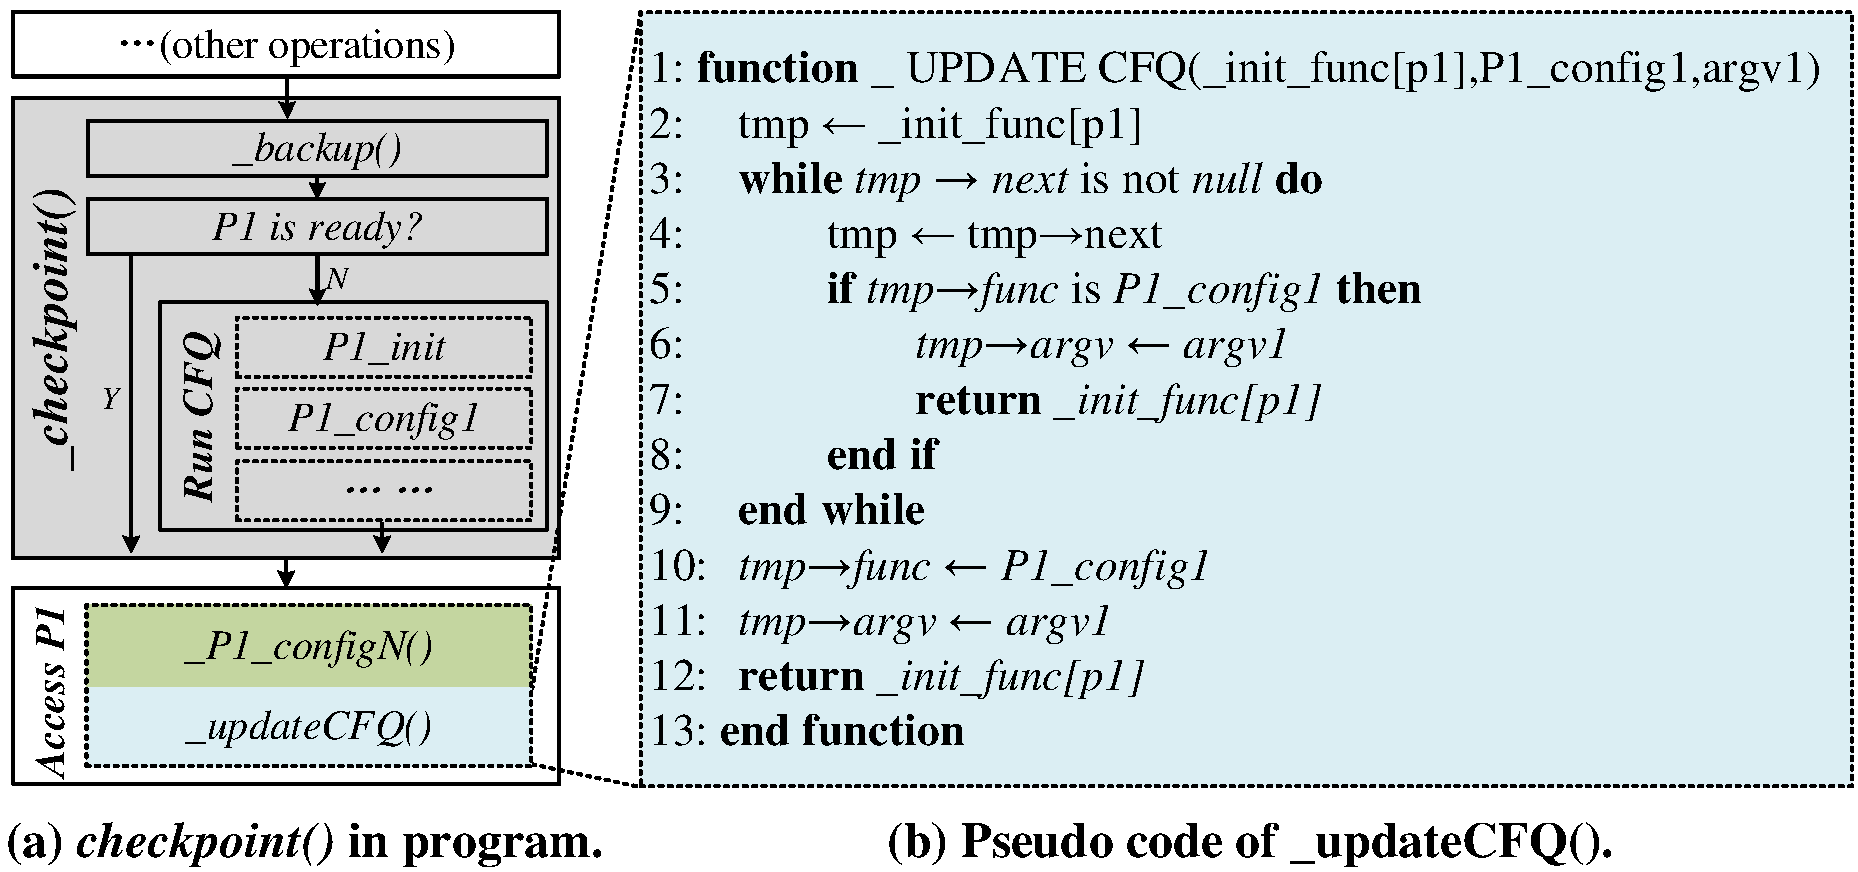
\includegraphics[width=0.48\textwidth]{Fig9_updateCFQ.pdf}
    \vspace{-15pt}
    \caption{Program when peripheral \emph{P1} is accessed. \emph{\_checkpoint()} is used to configure \emph{P1} and \emph{\_updateCFQ()} is used to track the latest configurations.}
    \vspace{-5pt}
    \label{fig:updateCFQ}
\end{figure}


\subsection{Peripheral Operation Restart} \label{sec:onlineRestart}
\vspace{-5pt}
%
After the peripherals are reconfigured, we are ready to restart the peripheral operations.
REMARK restarts the peripheral operations from peripheral checkpoints with the help of PRM (described in Sec.~\ref{sec:hardware}) and Initiator.


\vspace{5pt}
\noindent\textbf{Restart Peripheral Operations by Initiator.} \\
As shown in Fig.~\ref{fig:Initiator}, Initiator is a program located in the top of instruction memory used to store the peripheral checkpoints.
It contains a list of peripheral checkpoints and a processor restore instruction.
Each peripheral checkpoint is a restart function, \emph{\_restart\_PT()}, which can restart a specific peripheral operation.
The queue is empty at the beginning and is dynamically updated by \emph{updateInitiator()} described in Sec.~\ref{sec:offlineTransformer}.

%
\begin{figure}[t]
    \centering
    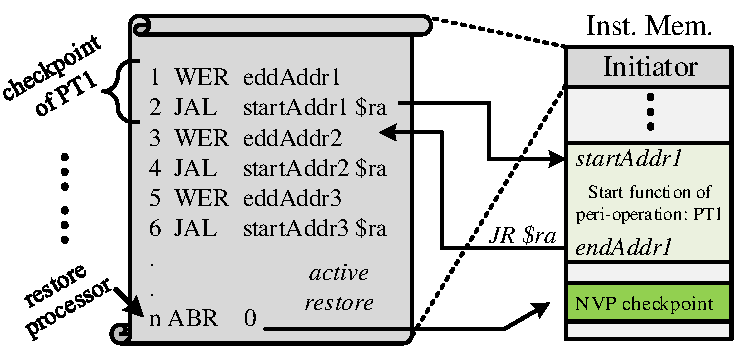
\includegraphics[width=0.48\textwidth]{Fig10_Initiator.pdf}
    \vspace{-15pt}
    \caption{Restart peripheral operations in Initiator.}
    \vspace{-1pt}
    \label{fig:Initiator}
\end{figure}

Each peripheral checkpoint consists of two instructions, \emph{WER} and \emph{JAL}.
Fig.~\ref{fig:Initiator} shows how to restart a peripheral operation, \emph{PT1}, with its checkpoint.
In this example, the first instruction writes the end address of \emph{PT1} start function, \emph{endAddr1}, into PRM.
The second instruction, \emph{JAL}, jumps to the start address of \emph{PT1} start function and links the address of the next instruction in Initiator into register \emph{\$ra}.
Then, the peripheral operation \emph{PT1} is restarted.
When the start function is finished, the PC counter reaches \emph{endAddr1}.
Then PRM automatically enable an \emph{JR \$ra} operation to return the program to Initiator and continue restarting the next peripheral operation.

\vspace{5pt}
\noindent\textbf{The Restart Flows after Power Failure.} \\
The restart flows are different from each other when power fails during different stages.
A peripheral operation can be decomposed into three stages: the starting stage, the execution stage, and the returning stage.
During the starting stage, the processor uses I/O instructions to start a peripheral operation.
The execution stage lasts until the returning interrupt is triggered.
Finally, the ISR returns the result to the processor in the returning stage.
The peripheral operation is completed only if the ISR is finished.

%
When power fails during the starting stage, the parallel peripheral operation has not been started.
No peripheral checkpoints are placed, and the processor only needs to rollback and re-run the starting stage.
Once the starting stage is completed, \emph{updateInitiator()} inserted during offline program transformation will place a peripheral checkpoint in Initiator.

When power fails during the execution stage, as shown in Fig.~\ref{fig:PeriRecoverProcedure} (a), the processor restores its state and the peripheral operations are restarted from their checkpoints individually.

When power fails during the returning stage, as shown in Fig.~\ref{fig:PeriRecoverProcedure} (b), the peripherals lose all the data and fail to return the results.
Therefore, the peripheral operations still need to be restarted.
Meanwhile, the processor needs to restore to the checkpoint located before the ISR, as discussed in Sec.~\ref{sec:offlineTransformer}.
When a successful ISR is completed, the peripheral operation is also finished.
Therefore, the peripheral checkpoint to restart this operation needs to be removed from Initiator by another \emph{\_updateInitiator()} function.

%
\begin{figure}[t]
    \centering
    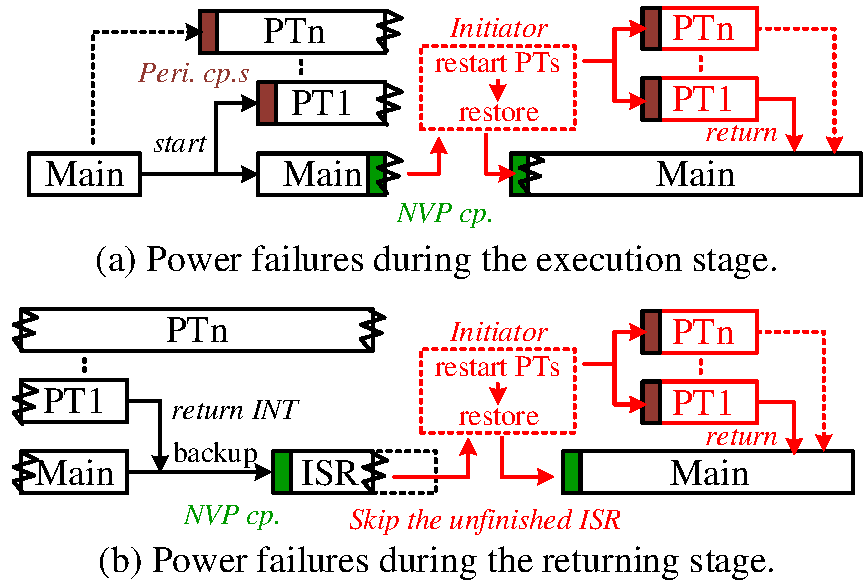
\includegraphics[width=0.45\textwidth]{Fig10_PeriRecoverProcedure.pdf}
    \vspace{-5pt}
    \caption{Power failures during the starting and the returning stage of peripheral operations.}
    \vspace{-5pt}
    \label{fig:PeriRecoverProcedure}
\end{figure}

% the resilience of REMARK
When power fails during the recover procedure, the devices can roll back to their checkpoints if these checkpoints are not crashed.
Therefore, completing the backup function is essential to ensure the validity of a checkpoint.
To guarantee the success of backup operation, NVP adopts a $4.7 \mu F$ on-chip capacitor.
In the hardware prototype of this paper, each backup operation consumes $77.69nJ$ in $7 \mu s$.
In this way, the system can safely backup whenever power fails.
